\documentclass[a4paper,11pt]{article}
\usepackage[T1]{fontenc}
\usepackage[utf8]{inputenc}
\usepackage{lmodern}
\usepackage{hyperref}
\usepackage{amsmath}
\usepackage{amssymb}
\usepackage{xcolor}
\usepackage{graphicx}
\usepackage{wrapfig}
\usepackage{caption}
\usepackage{multicol}


\hypersetup{
  colorlinks=true,
  linkcolor=gray,
  urlcolor=blue
}

\title{Parallel Solution of Laplace's Equation}
\author{Leo Unbekandt}

\begin{document}

\maketitle
\tableofcontents

\begin{abstract}
  The main goal of this work is to develop a parallel way to solve numerically Laplace's Equation by using OpenMPI,
  and to analyze how this process accelerates the computation compare to the serial way to do, and how exact are the
  results compare to the analytical solution. The using method in this project must have been Jacobi with red-black
  ordering. However there is no interest in doing red-black ordering with Jacobi as we have to keep the old matrix in
  memory, that's why I've decided to use Gauss Seidel method associated with red-black ordering.
  
  The complete source code of this project may be found on Github: \url{https://github.com/Soulou/HPC_Assignment}
  It includes the analytical, the serial and the parallel methods, and additionaly the \LaTeX \hspace{5pt} source code of this
  report.
\end{abstract}

\section{The analytical solution}
\subsection{Solving the equation by using Fourier series}

Finding the analytical solution basically consists in solving:
2$$\frac{\partial^2 \phi}{\partial y^2} + \frac{\partial^2 \phi}{\partial x^2} = 0 \hspace{2em} x \in [0,1], y \in [0,1]$$

\noindent The homogeneous boundary conditions are:
$$\phi(x,0) = 0 \hspace{3em} \phi(x,1) = 0 \hspace{3em} \phi(1,y) = 0$$

\noindent The inhomogeneous boundary condition is:
$$\phi(0,y) = sin^2(\pi y)$$

\noindent The separating the variables, we obtain $\phi(x,y) = X(x)Y(y)$, so Laplace's equation becomes:
$$\frac{1}{X}\frac{\partial^2 X}{\partial x^2} + \frac{1}{Y}\frac{\partial^2 Y}{\partial y^2} = 0$$

\noindent Let: $$\frac{1}{Y}\frac{\partial^2 Y}{\partial y^2} = - k^2 \Leftrightarrow Y(y) = A_1\cos(k y) + B_1\sin(k y)$$ 
So:
\begin{align*}
  \frac{1}{X}\frac{\partial^2 X}{\partial x^2} = k^2 \Leftrightarrow X(x) & = A_2\cosh(k x) + B_2\sinh(k x) \\
  Or: X(x) & = A_2\cosh(k (x-1)) + B_2\sinh(k (x-1))
\end{align*}

\noindent This second expression works better with $X(0) = 0$ as boundary condition. As a result we have:
$$\phi(x,y) = [ A_1\cos(k y) + B_1\sin(k y)][A_2\cosh(k (x-1)) + B_2\sinh(k (x-1))]$$

\noindent Thanks to our boundary conditions we deduce that
$$Y(0) = 0 \Rightarrow A_1=0 \hspace{2em} Y(1) = 0 \Rightarrow k=n \pi \hspace{2em} X(1) = 0 \Rightarrow A_2 = 0$$

\noindent Finally we get:
\begin{align*}
  \phi_n(x,y) & = B_n \sin(n \pi y)\sinh(n \pi (x-1)) & for\hspace{5pt}n \in \mathbb{N}^{+*} \\
  \phi_n(x,y) & = \sum_{n = 1}^{\infty}{B_n \sin(n \pi y)\sinh(n \pi (x-1))} & (by\hspace{5pt}superposition)
\end{align*}

\noindent Thanks to the inhomogeneous boundary condition we have:
\[
  \phi(0, y) = \sum_{n = 1}^{\infty}{B_n sin(n \pi y)\sinh(-n \pi)}
\]
The Fourier coefficient is now $B_n \sinh(-n \pi)$:
\begin{align*}
  B_n \sinh(-n \pi) & = \int_{0}^{1}{\sin^2(\pi y)\sin(n \pi y)dy} \\
  B_n & = \frac{2(\cos(\pi n) - 1)}{\pi(n^3 - 4n)\sinh(-n \pi)}
\end{align*}

\subsection{Implementation of the solution}
  The implementation has been done with the C programming language. The only constraint of using this language is
  that the result formula contains $\sinh(-n \pi)$. When $n$ gets bigger, a primitive variable type (double, long double)
  is not able anymore to have enough precision to compute correct results. This is why I've used the library
  GNU MPFR which is used to manipulate with high precision floating point numbers.
  
\subsection{Illustration of the analytical solution}

\begin{figure}[h!]
  \centering
  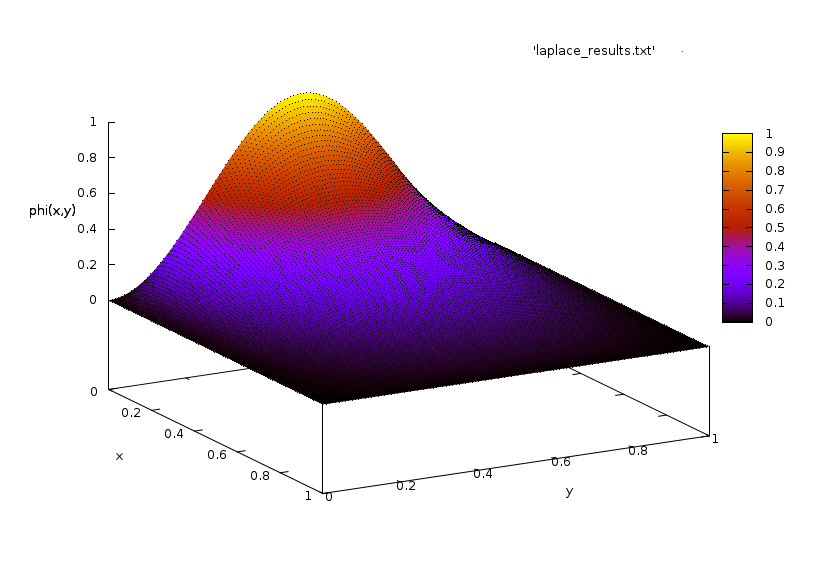
\includegraphics[width=0.8\textwidth]{images/analytical.png}
  \caption{Representation of $\phi(x,y)$ for a stepsize of 1/120}
\end{figure}

\section{The numerical solution - serial computation}
\subsection{Implementation}

\begin{wrapfigure}[12]{r}{0.45\textwidth}
  \hspace{2em}
  \vspace{1em}
  \caption{Finite difference stencil}
  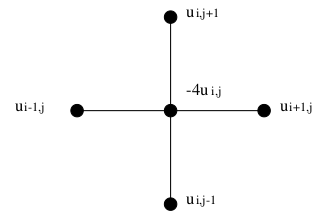
\includegraphics[width=0.45\textwidth]{images/gauss-seidel.png}
\end{wrapfigure}

The implementation of Gauss-Seidel method consists in a successive number of iterations of the following formula.

$$\phi^{k+1}_{i,j} = \frac{1}{4}(\phi^{k}_{i+1,j} + \phi^{k+1}_{i-1,j} + \phi^{k}_{i,j+1} + \phi^{k+1}_{i,j-1})$$
$$i \in [2;k-1], j \in [2;k-1]$$

This is really convenient to implement, because by iterating by line as it is showed in the following schema, when
we calculate the point $o22$ we already have $\phi^{k+1}_{i-1,j}$ and $\phi^{k+1}_{i,j-1}$ because they have been
computed previously. The consequence is that we don't need to keep a copy of the old matrix in memory, we can iterate
on in directly.
  
\begin{verbatim}
                 _____________________________
                |                             |
                | f   0   0   0   ...   0   0 |
                | f  n11 n12 n13  ...  n1k  0 |
                | f  n21 o22 o23  ...  o2k  0 |
                |                             |
                |                             |
                |           .........         |
                |                             |
                |                             |
                |                             |
                |_____________________________|
\end{verbatim}

Another important point, is the stopping condition. The following choice has been done: after each iteration we are looking
at the norm of the difference between the newly computed matrix and the previous one and we compare it to a certain tolerance
the user has to give as argument to the software.

\[
  ||\phi^{k+1} - \phi^{k}|| < \epsilon
\]

\subsection{Aspect of the results}

The results look similar as the results obtained in the analytical computation:

\begin{figure}[h!]
  \centering
  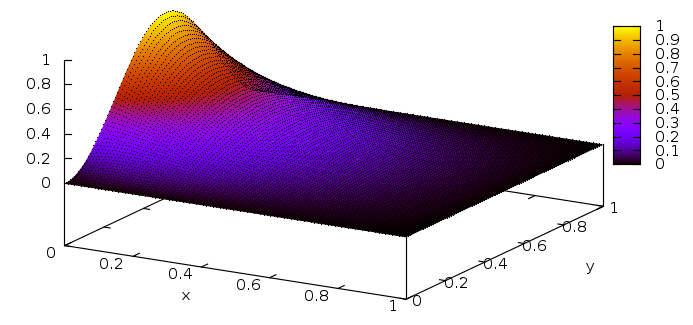
\includegraphics[width=0.45\textwidth]{images/serial-results.png}
\end{figure}

\subsection{Validation of the implementation}

To know if the results are accurate we need to compare them to the results of the analytical solution. In order to
achieve that, I've developed a small script: \texttt{diff\_results.rb} which compares two result files by calculating the
difference of each $\phi(x,y)$ and finally printing the average difference in percents. The following table shows the difference
between the analytical implementation and the Gauss-Seidel serial version, for different sizes of domain and different error tolerances
\footnote{Data generated by: analytical\_serial\_diff.sh}.


\begin{itemize}
\item{N: Number of steps/size of the result matrix}
\item{\=e: Average error}
\item{t: convergence tolerance}
\end{itemize}

\begin{center}
\captionof{table}{Difference between analytical and serial solutions}
\vspace{1em}
\begin{tabular}{c | c | c | c | c}
N & \=e ,t = $10^{-2}$ & \=e, t = $10^{-3}$ & \=e, t = $10^{-4}$ & \=e, t = $10^{-5}$ \\
20 & 0.1822 & 0.1325 & 0.1234 & 0.1227 \\
40 & 0.2170 & 0.1086 & 0.0737 & 0.0708 \\
60 & 0.2626 & 0.1091 & 0.0554 & 0.0500 \\
80 & 0.3004 & 0.1171 & 0.0465 & 0.0388 \\
100 & 0.3206 & 0.1228 & 0.0421 & 0.0320 \\
\end{tabular}
\end{center}

There are different things we can observe in this table. First, whatever is the size of the Domain, we can observe that
the precision of the results is better when the tolerance is decreasing. Then, the results look accurate when the 
convergence tolerance is small enough. Actually when $t = 10^{-5}$ and $N \geq 60$, the numerical results are less
than 5\% different from the analytical one. Finally we can also see that the bigger the domain, the small the required
tolerance has to be to obtain good results. As a result we can validate this way to measure the error and to detect the
convergence.

\clearpage

\section{OpenMPI - parallel computation}

\subsection{Computational domain decomposition}

To divide a matrix, there are two main solutions:
\begin{itemize}
\item{Panels:
\begin{multicols}{2}
\begin{verbatim}
 ____________________
|      |      |      |
|      |      |      |
|      |      |      |
|      |      |      |
|      |      |      |
|      |      |      |
|      |      |      |
|      |      |      |
|______|______|______|
\end{verbatim}
\vspace{1em}
\begin{verbatim}
 ____________________
|                    |
|                    |
|____________________|
|                    |
|                    |
|____________________|
|                    |
|                    |
|____________________|
\end{verbatim}

\end{multicols}
}
\item{Squares:
\begin{multicols}{2}
\begin{verbatim}
 ____________________
|          |         |
|          |         |
|          |         |
|          |         |
|----------|---------|
|          |         |
|          |         |
|          |         |
|__________|_________|
\end{verbatim}

\begin{verbatim}
 ____________________
|      |      |      |
|      |      |      |
|______|______|______|
|      |      |      |
|      |      |      |
|______|______|______|
|      |      |      |
|      |      |      |
|______|______|______|
\end{verbatim}
\end{multicols}
}
\end{itemize}

As shown above, the panels decomposition may be horizontal or vertical. Fondamentaly there
is no difference between their characteristics, their are as many value to calculate and to
exchange. However their is one difference which is linked to how caching is managed on the
computing nodes. In our case the cache is storing lines, that's why it is much better to use
horizontal panels than vertical.

\subsection{Data exchange and halo nodes}

The main advantage of the panels compare to the squares is that each process only need to
communicate with a maximum of 2 other instances (the one above and the one underneath).
Even if by dividing the domain in squares, some processes would need to communicate with
4 other nodes, the amount of data which has to be exchanged by each process is smaller:

\begin{multicols}{2}
\begin{verbatim}
 ____________________
|          |         |
|          |         |
|          |         |
|          |         |
|----------|---------|
|          |         |
|          |         |
|          |         |
|__________|_________|
\end{verbatim}
\begin{verbatim}
 ____________________
|                    |
|____________________|
|                    |
|____________________|
|                    |
|____________________|
|                    |
|____________________|
\end{verbatim}
\end{multicols}




\end{document}
